\chapter{Installing OpenDQ}
\label{sec:03-installing}
This section explains how to install the software that is required to compile, run and debug the OpenDQ project on a computer. 

%%
% Prerequisites
%%
\section{Prerequisites}
OpenDQ requires Ubuntu 14.04 to operate, either the 32 bit or the 64 bit version. The reason why Ubuntu 14.04 LTS is selected as the supported operating system is because it is a LTS (Long Term Support) release, meaning that it is more stable that regular releases and that it will remain supported until April 2019. However, OpenDQ is also known to run on other versions of the GNU/Linux operating system, as well as on Windows and MacOS operating systems. However, these platforms are not supported by the current documentation.

The remaining of this subsection assumes that Ubuntu 14.04 LTS is installed in a computer that has access to the Internet. If you do not have Ubuntu 14.04 LTS installed on your computer, please download it (http://www.ubuntu.com/download) and install it in the computer prior to continuing. Please notice that it is also possible to install Ubuntu 14.04 LTS and OpenDQ in a virtual environment, i.e. VMWare Player or VMWare Workstation.

Once Ubuntu 14.04 is installed in a computer or virtual machine, please make sure that the operating system is updated with the latest security patches and software versions by executing the following commands. If the process is successful, a screen similar to Figure~\ref{fig:05-update} will be displayed.

\begin{verbatim}
sudo apt-get update
sudo apt-get dist-upgrade
\end{verbatim}

% Updating the Ubuntu 14.04 LTS operating system.
\begin{figure}[!ht]
    \centering
	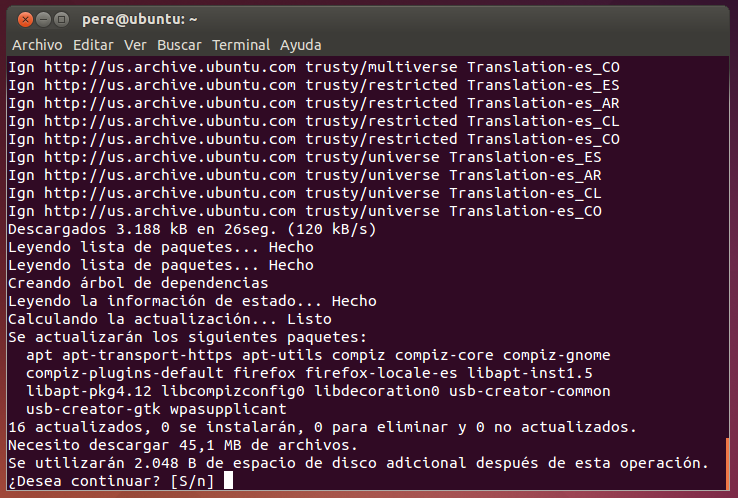
\includegraphics[width=0.75\linewidth]{05-update}
    \caption{Updating the Ubuntu 14.04 LTS operating system.}
    \label{fig:05-update}
\end{figure}

After installing and updating the operating system, proceed to install the remaining software required to compile, run and debug the OpenDQ project, as described in the following subsections.

%%
% Git
%%
\section{Git}
The OpenDQ project uses Git as the version control system to manage the source code. To install git and the related dependencies execute the following command on a terminal window.

\begin{verbatim}
sudo apt-get install git
\end{verbatim}

%%
% Python
%%
\section{Python}
The OpenDQ project requires Python 2.7 and certain libraries, i.e., pyserial, numpy, scipy and matplotlib. To install Python and the related dependencies execute the following command on a terminal window.

\begin{verbatim}
sudo apt-get install python python-serial python-numpy python-scipy python-matplotlib
\end{verbatim}

%%
% Toolchain
%%
\section{Toolchain}
The OpenDQ project requires an arm-none-eabi-gcc toolchain to cross-compile the C source code for the ARM Cortex-M architecture. To install the arm-none-eabi-gcc toolchain execute the following commands on a terminal window.

\begin{verbatim}
sudo apt-get remove binutils-arm-none-eabi gcc-arm-none-eabi
sudo add-apt-repository ppa:terry.guo/gcc-arm-embedded
sudo apt-get update
sudo apt-get install build-essential gcc-arm-none-eabi=4.9.3.2015q1-0utopic14
\end{verbatim}

\section{Segger J-Link}
The OpenDQ project requires the Segger J-Link software to load and debug the binaries for the ARM Cortex-M architecture. To install the Segger J-Link software go to the follwing link (https://www.segger.com/jlink-software.html) and download the latest TGZ archive for the J-Link software for your operating system, i.e. Linux 32 or 64 bits. Currently the version is Linux v.498b.

Once downloaded, uncompress it and copy it to the $/opt$ directory by executing the following commands.
\begin{verbatim}
tar xzvf Jlink_Linux_V498b_x86_64.tgz
sudo mkdir /opt/segger
sudo mv JLink_Linux_V498b_x86_64 /opt/segger/jlink
\end{verbatim}

Finally, add the directory to the $PATH$ variable by editing the $.bashrc$ file in the user home directory.